\chapter{Subgrupos, Generadores, Retículos y Grupos cíclicos}
\begin{definicion}[Subgrupo]
    Dados dos grupos $G$ y $H$, decimos que $H$ es un subgrupo de $G$, denotado por $H < G$, si $H\subseteq G$ y la aplicación de inclusión\footnote{Viene dada por $i(x) = x$, para todo $x\in H$.} $i:H\to G$ es un homomorfismo de grupos.
\end{definicion}

\begin{observacion}
    Dado un grupo $(G,\ast,e)$, este tendrá siempre dos subgrupos:
    \begin{itemize}
        \item $(\{e\},\ast,e)$, al que llamaremos \underline{subgrupo trivial}.
        \item El propio $(G, \ast, e)$
    \end{itemize}
\end{observacion}

\begin{definicion}
    Sea $H$ un subgrupo de otro $G$, diremos que $H$ es un \underline{subgrupo impropio} de $G$ si $H$ es el grupo trivial o el propio $G$. En otro caso, diremos que $H$ es un \underline{subgrupo propio} de $G$.
\end{definicion}

\begin{notacion}
    Recordamos la notación que ya usábamos en Álgebra I para, fijado $n\in \mathbb{N}\setminus\{0\}$, denotar a todos los múltiplos de $n$ en $\mathbb{Z}$:
    \begin{equation*}
        n\mathbb{Z} = \{nm \mid m\in \mathbb{Z}\}
    \end{equation*}
\end{notacion}

\begin{ejemplo}
    Vemos claramente que:
    \begin{enumerate}
        \item $(\mathbb{Z},+) < (\mathbb{Q},+) < (\mathbb{R}, +)$
        \item $\{r^k \mid k\leq n, r\in D_n\} < D_n$ 
        \item $n\mathbb{Z} < \mathbb{Z}$ para todo $n\in \mathbb{N}$.
        \item $\SL_n(\mathbb{F}) < \GL_n(\mathbb{F})$
        \item $(\mathbb{Q}^\ast, \cdot) \not< (\mathbb{R}, +)$ No es un subgrupo, ya que $i(1) = 1 \neq 0$.
        \item $(\mathbb{Z}^+, +) \not< (\mathbb{Z}, +)$, ya que $(\mathbb{Z}^+, +)$ no es un grupo.
        \item $D_6 \not< D_8$, ya que $D_6\nsubseteq D_8$.
    \end{enumerate}
\end{ejemplo}

\begin{observacion}
    Si $G$, $H$ y $T$ son grupos de forma que $G < H < T$, entonces $G < T$.
    \begin{proof}
        La transitividad de $\subseteq $ nos da que $G\subseteq H\subseteq T$. Por otra parte, como las inclusiones $j:G\to H$ y $k:H\to T$ son homomorfismos, tendremos que $i=k\circ j:G\to T$ es un homomorfismo.
    \end{proof}
\end{observacion}

\begin{prop}\label{prop:carac_subgrupo}
    Sea $G$ un grupo y $\emptyset \neq H \subseteq G$, entonces son equivalentes:
    \begin{enumerate}
        \item[$i)$] $H < G$
        \item[$ii)$] Se verifican:
            \begin{enumerate}[label=(\alph*)]
                \item Si $x,y\in H$ entonces $xy\in H$.
                \item $1\in H$.
                \item Si $x\in H$, entonces $x^{-1}\in H$.
            \end{enumerate}
        \item[$iii)$] Si $x,y\in H$, entonces $xy^{-1}\in H$.
    \end{enumerate}
    \begin{proof}
        Veamos las implicaciones de forma cíclica:
        \begin{description}
            \item [$i)\Longrightarrow ii)$] Como $H$ es un grupo, por su definición se han de cumplir $(a)$, $(b)$ y $(c)$.
            \item [$ii)\Longrightarrow iii)$] Si $x,y\in H$, entonces $y^{-1}\in H$, por lo que tendremos que $xy^{-1}\in H$.
            \item [$iii)\Longrightarrow i)$] Como $\emptyset \neq H$, existirá al menos un $x\in H$, por lo que $xx^{-1} = 1 \in H$.
                Además, si $x\in H$ también tendremos que $1x^{-1} = x^{-1}\in H$.
                Para ver que $H$ es un grupo, tan solo nos falta ver que su operación interna está bien definida; es decir, que si $x,y\in H$, entonces $xy\in H$. Dados $x,y\in H$, tendremos que $y^{-1}\in H$, por lo que:
                \begin{equation*}
                    xy = x(y^{-1})^{-1} \in H
                \end{equation*}
                
                Con esto tenemos ya que $H$ es un grupo. Al considerar en $H$ la misma operación que en $G$, tenemos directamente que $i:H\to G$ es un homomorfismo, ya que $id:H\to H$ es un homomorfismo y al extender el codominio para considerar la aplicación inclusión $i$, seguirá siendo un homomorfismo\footnote{Notemos que si en $H$ tenemos una operación distinta que en $G$ esto no siempre será cierto y habrá que comprobar que $i:H\to G$ es un homomorfismo.}.\\

                \noindent
                Esta observación la usaremos con frecuencia en toda la asignatura: cada vez que tengamos $G$ un grupo y $H\subseteq G$, como casi siempre consideraremos en $H$ la misma operación que en $G$, bastará simplemente demostrar también que $H$ es un grupo, para así concluir que $H < G$.
        \end{description}
    \end{proof}
\end{prop}

\begin{prop}
    Sea $G$ un grupo finito y $\emptyset \neq H \subseteq G$, entonces son equivalentes:
    \begin{enumerate}
        \item[$i)$] $H < G$
        \item[$ii)$] Si $x,y\in H$, entonces $xy\in H$
    \end{enumerate}
    \begin{proof}
        Veamos las dos implicaciones:
        \begin{description}
            \item [$i)\Longrightarrow ii)$] Se verifica por ser $H$ un grupo.
            \item [$ii)\Longrightarrow i)$] Como $G$ es finito, por la Proposición~\ref{prop:orden_grupo}, para todo $x\in G$ existirá $n>0$ de forma que $x^n = 1$, por lo que $x^{-1} = x^{n-1}$. De esto deducimos que $x^{-1}\in H$ y que $1=xx^{-1}\in H$. Por la Proposición~\ref{prop:carac_subgrupo}, $H<G$.
        \end{description}
    \end{proof}
\end{prop}

\begin{ejemplo}
    Se deja como ejercicio comprobar que:
    \begin{enumerate}
        \item $A_n < S_n$
        \item Todo subgrupo de $\mathbb{Z}$ es de la forma $n\mathbb{Z}$ con $n\in \mathbb{N}$.
        \item $V<S_4$
        \item Si $n\mid m$, entonces $D_n < D_m$
    \end{enumerate}
\end{ejemplo}

\begin{definicion}
    Sea $G$ un grupo, $f:G\to G'$ una aplicación, y $H\subseteq G$, $H'\subseteq G'$, definimos:
    \begin{itemize}
        \item El conjunto imagen directa de $H$ por $f$ como el conjunto:
            \begin{equation*}
                f_\ast(H) = \{f(x) \mid x\in H\}\subseteq G'
            \end{equation*}
        \item El conjunto imagen inversa de $H'$ por $f$ como el conjunto:
            \begin{equation*}
                f^\ast(H') = \{x\in G \mid f(x) \in H'\}\subseteq G
            \end{equation*}
    \end{itemize}
\end{definicion}

\begin{prop}\label{prop:imagen_directa}
    Sea $f:G\to G'$ un homomorfismo de grupos, entonces: 
    \begin{enumerate}
        \item[$i)$] Si $H<G$, entonces $f_\ast(H)< G'$ 
        \item[$ii)$] Si $H'<G'$, entonces $f^\ast(H')< G$
    \end{enumerate}
    \begin{proof}
        Demostramos las dos implicaciones:
        \begin{enumerate}
            \item[$i)$] Sean $x,y\in f_\ast(H)$, entonces $\exists a,b\in H$ de forma que $x=f(a), y=f(b)$. Como $H$ es un subgrupo de $G$, tendremos que $ab^{-1}\in H$, por lo que:
            $$f(ab^{-1}) = f(a){f(b)}^{-1} = xy^{-1}\in f_\ast(H)$$
            Concluimos que $f_\ast(H)$ es un subgrupo de $G'$.
            \item[$ii)$] Sean $x,y\in f^\ast(H')$, entonces $a=f(x), b=f(y)\in H'$. Por ser $H'$ un subgrupo de $G'$, tendremos que
            $$ab^{-1} = f(x){f(y)}^{-1}=f(xy^{-1})\in H'$$
            Por tanto, ${xy^{-1}\in f^\ast(H')}$. Concluimos que $f^\ast(H')$ es un subgrupo de $G$.
        \end{enumerate}
    \end{proof}
\end{prop}

\begin{prop}\label{prop:interseccion_subgrupos}
    Sea $\{H_i\}_{i \in I}$ una familia de subgrupos de $G$, entonces la intersección de todos ellos sigue siendo un subgrupo de $G$:
    \begin{equation*}
        \bigcap_{i \in I} H_i < G
    \end{equation*}
    \begin{proof}
        En primer lugar, como $H_i < G$ para todo $i \in I$, se ha de verificar que $1\in H_i$ $\forall i \in I$, por lo que $1\in \bigcap\limits_{i \in I} H_i \neq \emptyset $. Como la intersección es no vacía, podemos pensar en aplicar el tercer punto de la Proposición~\ref{prop:carac_subgrupo} para comprobar que es un subgrupo de $G$.\\

        \noindent
        Para ello, sean $x,y\in \bigcap\limits_{i \in I}H_i$, entonces $x,y\in H_i$ para todo $i \in I$, por lo que por ser $H_i < G$, tendremos que $xy^{-1}\in H_i$ $\forall i \in I$, luego:
        \begin{equation*}
            xy^{-1} \in \bigcap_{i \in I}H_i
        \end{equation*}
        Concluimos que $\bigcap\limits_{i \in I}H_i$ es un subgrupo de $G$.
    \end{proof}
\end{prop}

\begin{ejemplo}
    En general, la unión de subgrupos no es un subgrupo:
    \begin{equation*}
        2\mathbb{Z} \cup 3\mathbb{Z}  \not< \mathbb{Z}
    \end{equation*}
    Ya que $2,3\in 2\mathbb{Z}\cup 3\mathbb{Z}$ y $2+3 = 5\notin 2\mathbb{Z}\cup 3\mathbb{Z}$.
\end{ejemplo}

\section{Generadores de subgrupos}
\begin{definicion}[Subgrupo generado]
    Sea $G$ un grupo y $S\subseteq G$, definimos el subgrupo generado por $S$ como el menor subgrupo de $G$ que contiene a $S$, es decir:
    \begin{equation*}
        \langle S \rangle  = \bigcap \{H < G \mid S\subseteq H\}
    \end{equation*}
\end{definicion}
\begin{observacion}
    Notemos que, gracias a la Proposición~\ref{prop:interseccion_subgrupos}, $\langle S \rangle $ efectivamente es un subgrupo de $G$.
\end{observacion}

\begin{prop}\label{prop:subgrupos_generados}
    Sea $(G,\cdot ,e)$ un grupo, $S\subseteq G$, entonces:
    \begin{itemize}
        \item Si $S = \emptyset $, entonces $\langle S \rangle = \{e\}$, el grupo trivial.
        \item Si $S\neq \emptyset $, entonces $\langle S \rangle = \{x_1^{\gamma_1}x_2^{\gamma_2}\ldots x_m^{\gamma_m} \mid m \geq 1, x_i \in S, \gamma_i \in \mathbb{Z}\}$
    \end{itemize} 
    \begin{proof}
        Distinguimos casos:
        \begin{itemize}
            \item Si $S=\emptyset $, entonces $\{e\} < G$ con $S\subseteq \{e\}$. Como $\{e\}$ solo tiene un elemento y todo subgrupo de $G$ contiene a $e$, concluimos que:
                \begin{equation*}
                    \langle S \rangle = \bigcap \{H < G \mid S \subseteq H\} = \{e\}
                \end{equation*}
            \item Si $S\neq \emptyset $, por doble inclusión:
                \begin{description}
                    \item [$\supseteq)$] Como $S\subseteq \langle S\rangle$ y $\langle S\rangle$ es un grupo, tendremos que:
                        \begin{equation*}
                            x_1^{\gamma_1}x_2^{\gamma_2}\ldots x_m^{\gamma_m} \in \langle S\rangle \qquad x_i \in S, \gamma_i \in \mathbb{Z}\quad \forall 1\leq i \leq m
                        \end{equation*}
                    \item [$\subseteq)$] Si llamamos $A$ al conjunto de la derecha, $A$ es un grupo, ya que si tomamos $a,b\in A$, existirán $x_1,\ldots,x_p$ y $y_1,\ldots,y_q$ en $S$ y $\gamma_1,\ldots,\gamma_p,\alpha_1,\ldots,\alpha_q\in \mathbb{Z}$ de forma que:
                        \begin{equation*}
                            a = x_1^{\gamma_1} \ldots x_p^{\gamma_p} \qquad b = y_1^{\alpha_1} \ldots y_q^{\alpha_q
}                        \end{equation*}
                        Por lo que
                        \begin{equation*}
                            ab^{-1} = x_1^{\gamma_1} \ldots x_p^{\gamma_p} y_q^{-\alpha_q} \ldots y_1^{-\alpha_1} \in A
                        \end{equation*}
                        Lo que demuestra que $A$ es un subgrupo de $G$. Además, como es claro que $S\subseteq A$, tenemos un grupo del que $S$ es subconjunto, por lo que por ser $\langle S\rangle$ el menor subgrupo que contiene a $S$, está claro que $\langle S\rangle\subseteq A$.\qedhere
                \end{description}
        \end{itemize}
    \end{proof}
\end{prop}

\begin{coro}
    Si $S\subseteq G$ de forma que $\langle S \rangle =G$, entonces $S$ es un conjunto de generadores de $G$.
    \begin{proof}
        Por la Proposición~\ref{prop:subgrupos_generados}, sabemos que si $\langle S \rangle = G$, entonces cualquier elemento $x\in G$ se puede expresar de la forma:
        \begin{equation*}
            x = x_1^{\gamma_1}x_2^{\gamma_2}\ldots x_m^{\gamma_m} \qquad x_i \in S, \gamma_i \in \mathbb{Z}, \quad \forall 1\leq i \leq m
        \end{equation*}
        Por lo que $S$ es un conjunto de generadores de $G$.
    \end{proof}
\end{coro}

\begin{ejemplo}
    Ejemplos interesantes de subgrupos generados por ciertos conjuntos son:
    \begin{enumerate}
        \item Si $S= \{r\}\subseteq D_n$, entonces $\langle S \rangle = \{1,r,r^2, \ldots, r^{n-1}\}$
        \item Si $S = \{s\}\subseteq D_n$, entonces $\langle S \rangle = \{1, s\}$
        \item Si $S = \{(1\ 2)(3\ 4), (1\ 3)(2\ 4)\}\subseteq S_4$, entonces $\langle S \rangle = V$
        \item Si $S=\{(x_1\ x_2\ x_3) \mid x_1<x_2<x_3\}\subseteq S_n$, entonces $\langle S \rangle = A_n$
        \item Si $S = \left\{\left(\begin{array}{cc}
            i & 0 \\
            0 & -i 
        \end{array}\right),  \left(\begin{array}{cc}
            0 & 1 \\
            -1 & 0 
        \end{array}\right)\right\}\subseteq \GL_2(\mathbb{C})$, entonces $\langle S \rangle < \GL_2(\mathbb{C})$.
    \end{enumerate}
\end{ejemplo}

En la Proposición~\ref{prop:interseccion_subgrupos} vimos que la intersección de una familia arbitraria de subgrupos era un subgrupo, mientras que con el ejemplo de $2\mathbb{Z}\cup 3\mathbb{Z}\subseteq \mathbb{Z}$, vimos que, en general, la unión de dos subgrupos no es un subgrupo. Sin embargo, cabe preguntarse de qué forma podemos hacer una operación parecida con subgrupos para sí obtener un subgrupo. De esto nace la siguiente definición.

\begin{definicion}[Compuesto]
    Sea $\{H_i\}_{i \in I}$ una familia de subgrupos de un grupo $G$, llamamos compuesto de los subgrupos $H_i$, denotado por $\bigvee\limits_{i \in I} H_i$, al subgrupo:
    \begin{equation*}
        \bigvee_{i \in I} H_i = \left\langle \bigcup_{i \in I} H_i \right\rangle 
    \end{equation*}
    Cuando tengamos un número finito de subgrupos $\{H_1, H_2, \ldots, H_n\}$, notaremos:
    \begin{equation*}
        H_1\lor H_2\lor \ldots \lor H_n
    \end{equation*}
\end{definicion}

Notemos que es natural la definición, ya que como la unión de subgrupos no es en general un subgrupo, buscamos el menor subgrupo que contenga a la unión de subgrupos, que por definición es el compuesto de la familia de subgrupos que queríamos unir.

\section{Retículo de subgrupos de un grupo}
Introduciremos ahora el concepto de retículo\footnote{Que en el contexto de teoría de conjuntos o del orden puede tener otra definición.}, estructura algebraica de gran interés que usaremos brevemente para trabajar de forma cómoda con el conjunto de todos los subgrupos de un grupo.

\begin{definicion}[Retículo]
    Un retículo es una tripleta $(L, \lor, \land)$ donde:
    \begin{itemize}
        \item $L$ es un conjunto no vacío.
        \item $\land$ y $\lor$ son dos operaciones\footnote{Es común referirse a $\lor$ por ``supremo'' y a $\land$ por ``ínfimo''.} binarias en $L$ que verifican las leyes:
            \begin{enumerate}
                \item[$i)$] Conmutativa:
                    \begin{equation*}
                        a\lor b = b\lor a \qquad a\land b = b\land a 
                    \end{equation*}
                \item[$ii)$] Asociativa:
                    \begin{equation*}
                        a\lor (b\lor c) = (a\lor b)\lor c \qquad a\land (b\land c) = (a\land b)\land c 
                    \end{equation*}
                \item[$iii)$] de Absorción: 
                    \begin{equation*}
                        a\lor (a\land b) = a \qquad a\land (a\lor b) = a 
                    \end{equation*}
                \item[$iv)$] de Idempotencia:
                    \begin{equation*}
                        a\lor a = a \qquad a\land a = a
                    \end{equation*}
            \end{enumerate}
    \end{itemize}
    En el caso de que $(L,\lor, \land)$ sea un retículo, es común definir una relación binaria notada por ``$\leq$'' y definida por:
    \begin{equation*}
        a\leq b \Longleftrightarrow a\lor b = b\Longleftrightarrow
        a\land b = a
    \end{equation*}
    donde para la segunda equivalencia hemos empleado la conmutatividad y la propiedad de absorción.
\end{definicion}

\begin{prop}
    Todo retículo $(L,\lor,\land)$ junto con la relación de orden $\leq$ que se define a partir de sus operaciones es un conjunto parcialmente ordenado.
    \begin{proof}
        Hemos de probar las propiedades:
        \begin{itemize}
            \item \underline{Reflexiva.} Por la propiedad de idempotencia, dado $a\in L$, tenemos que:
                \begin{equation*}
                    a\lor a = a \Longrightarrow a\leq a
                \end{equation*}
            \item \underline{Antisimétrica.} Sean $a,b\in L$ de forma que $a\leq b$ y $b\leq a$. Por definición de $\leq$, tenemos que:
                \begin{equation*}
                    a\lor b = b \qquad b\lor a = a
                \end{equation*}
                Y aplicando la conmutatividad de $\lor$ llegamos a que:
                \begin{equation*}
                    a = a\lor b = b\lor a = b
                \end{equation*}
            \item \underline{Transitiva.} Sean $a,b,c\in L$ de forma que $a\leq b$ y $b\leq c$, es decir, $a\lor b = b$ y $b\lor c = c$, entonces:
                \begin{equation*}
                    a\lor c = a\lor (b\lor c) = (a\lor b)\lor c = b\lor c = c
                \end{equation*}
                De donde deducimos que $a\leq c$.
        \end{itemize}
    \end{proof}
\end{prop}

\begin{ejemplo}
    Ejemplos de retículos son:
    \begin{enumerate}
        \item El retículo endoplasmático rugoso.
        \item Dado un número $n\in \mathbb{N}$, el conjunto de divisores de $n$:
            \begin{equation*}
                D(n) = \{m\in \mathbb{N}: m \text{\ divide a\ } n\}
            \end{equation*}
            Junto con las operaciones de:
            \begin{align*}
                a\lor b &= \mcm(a,b) \\
                a\land b &= \mcd(a,b) 
            \end{align*}
            forma un retículo\footnote{Es un buen ejercicio comprobarlo.}. En este, la relación de orden que obtenemos es la de ``ser divisor de''; es decir, si $a,b\in D(n)$, entonces:
            \begin{equation*}
                a\leq b \Longleftrightarrow a\mid b
            \end{equation*}
        \item En la asignatura LMD vimos que los álgebras de Boole eran retículos.
    \end{enumerate}
\end{ejemplo}

\begin{lema}
    Sea $G$ un grupo y $T, U < G$, entonces:
    \begin{equation*}
        \langle \langle T \rangle \cup U \rangle  = \langle T\cup U \rangle 
    \end{equation*}
    \begin{proof}
        Haǵamoslo por doble inclusión:
        \begin{description}
            \item [$\supseteq)$] Basta ver que:
                \begin{equation*}
                    T\subseteq \langle T \rangle \Longrightarrow T\cup U \subseteq \langle T \rangle \cup U \Longrightarrow \langle T\cup U \rangle \subseteq \langle \langle T \rangle \cup U \rangle 
                \end{equation*}
            \item [$\subseteq)$] Sea $x\in \langle \langle T \rangle \cup U \rangle $, entonces existirán $\alpha_1,\ldots,\alpha_n\in \langle T \rangle $, $u_1,\ldots,u_m\in U$ y $\gamma_1,\ldots,\gamma_{n+m}\in \mathbb{Z}$ de forma que:
                \begin{equation*}
                    x = \alpha_1^{\gamma_1}\ldots \alpha_n^{\gamma_n}u_1^{\gamma_{n+1}}\ldots u_m^{\gamma_{n+m}}
                \end{equation*}
                Pero por ser $\alpha_1,\ldots,\alpha_n\in \langle T \rangle $, podemos encontrar $t_{ij}\in T$ y $\delta_{ij}\in \mathbb{Z}$ de forma que:
                \begin{align*}
                    \alpha_1 &= t_{11}^{\delta_{11}}\ldots t_{1n_1}^{\delta_{1n_1}} \\
                             &\vdots \\
                    \alpha_n &= t_{n1}^{\delta_{n1}}\ldots t_{nn_n}^{\delta_{nn_n}}
                \end{align*}
                Por lo que:
                \begin{equation*}
                    x = t_{11}^{\delta_{11}}\ldots t_{1n_1}^{\delta_{1n_1}} \ldots t_{nn_n}^{\delta_{nn_n}}u_1^{\gamma_{n+1}}\ldots u_m^{\gamma_{n+m}} \in \langle T\cup U \rangle 
                \end{equation*}
        \end{description}
    \end{proof}
\end{lema}

\begin{prop}
    Sea $G$ un grupo, si definimos el conjunto de subgrupos de $G$:
    \begin{equation*}
        \Lambda_G = \{H \subseteq G \mid H < G\}
    \end{equation*}
    Se verifica que $\Lambda_G$ es un retículo, junto con las operaciones:
    \begin{align*}
        T \lor U &= \langle T\cup U \rangle  \\
        T \land U &= T\cap U
    \end{align*}
    Además, la relación de orden en $\Lambda_G$ es $\subseteq $.
    \begin{proof}
        De Álgebra I ya sabemos que la intersección de conjuntos es conmutativa, asociativa y que tiene la propiedad de idempotencia. Veamos estas para el compuesto de dos subgrupos, que se deducen a partir de las propiedades conmutativa, asociativa y de idempotencia para la unión de dos conjuntos:
        \begin{itemize}
            \item \underline{Conmutativa.} Sean $T,U\in \Lambda_G$:
                \begin{equation*}
                    T\lor U = \langle T\cup U \rangle  = \langle U\cup T \rangle  = U\lor T
                \end{equation*}
            \item \underline{Asociativa.} Sean $T,U,V \in \Lambda_G$:
                \begin{multline*}
                    T\lor(U\lor V) = T\lor \langle U\cup V \rangle  = \langle T\cup \langle U\cup V \rangle  \rangle  \AstIg \langle T\cup U\cup V \rangle  \\ \AstIg \langle \langle T\cup U \rangle \cup V \rangle  = \langle T\cup U \rangle \lor V = (T\lor U)\lor V
                \end{multline*}
                Donde en $(\ast)$ hemos aplicado el Lema anterior.
            \item \underline{Idempotencia.} Sea $T\in \Lambda_G$:
                \begin{equation*}
                    T\lor T = \langle T\cup T \rangle  = \langle T \rangle  \AstIg T
                \end{equation*}
                Donde en $(\ast)$ hemos usado que $T$ es un grupo, por ser subgrupo de $G$.
        \end{itemize}
        Finalmente, nos queda comprobar las \underline{propiedades de absorción}. Para ello, sean $T,U\in \Lambda_G$:
        \begin{gather*}
            T\lor (T\cap U) = \langle T\cup (T\cap U) \rangle = \langle (T\cup T) \cap (T\cup U) \rangle  = \langle T\cap (T\cup U) \rangle = \langle T \rangle  = T \\
            T\cap (T\lor U) = T\cap \langle T\cup U \rangle = T
        \end{gather*}
        Para ver que la relación de orden es $\subseteq $, notemos que si $T,U\in \Lambda_G$, entonces:
        \begin{equation*}
            A\subseteq B \Longleftrightarrow A \cap B = A
        \end{equation*}
        Que es como se define la relación de orden para los retículos.
    \end{proof}
\end{prop}

Al trabajar con retículos, una estructura que surge de forma natural son los diagramas de Hasse, que nos permiten comprender mucho mejor la estructura de un retículo concreto.

\begin{definicion}[Diagrama de Hasse]
    Sea $(L,\leq)$ un conjunto finito parcialmente ordenado, definimos su diagrama de Hasse como el grafo dirigido $(V, E)$ donde:
    \begin{itemize}
        \item Los vértices son cada uno de los elementos de $L$, es decir: $V = L$.
        \item Dados dos vértices $a,b\in V$ con $a\neq b$, tendremos una arista de $a$ a $b$ ($a\to b$) si $a\leq b$ y no existe ningún elemento $c\in V$ con $a\neq c\neq b$ de forma que $a\leq c\leq b$.

            Es decir, escribiremos $a\to b$ en el caso en el que $a\leq b$, obviando los ciclos (ya que $\leq$ es una relación reflexiva) y las relaciones que puedan deducirse de la transitividad de $\leq$: si $a\leq b$ y $b\leq c$, no consideraremos la arista $a\to c$.
    \end{itemize}
\end{definicion}

\begin{notacion}
    Por comodidad y claridad a la hora de dibujar los diagramas de Hasse, no dibujaremos grafos dirigidos, sino lo que haremos será primero ordenar los vértices por ``niveles'' en función de la cardinalidad de los subgrupos: colocaremos en el nivel más bajo el menor subgrupo del grupo que consideremos (notemos que siempre será el subgrupo trivial $\{e\}$) e iremos subiendo en niveles por la cardinalidad del subgrupo, hasta llegar al nivel superior, donde colocaremos al grupo de mayor cardinal (que coincidirá con el grupo que consideramos inicialmente).

    En segundo lugar, uniremos aquellos nodos que han de estar unidos mediante aristas no dirigidas (entendiendo que en realidad son aristas dirigidas, todas ellas apuntando hacia arriba, que es donde están los conjuntos más grandes).\\

    De esta forma, tendremos el diagrama de Hasse ordenado por niveles, donde podremos ver ``qué tan grande'' es cada subgrupo, así como las relaciones de inclusión entre ellos gracias a las aristas.
\end{notacion}

\subsection{Ejemplos}
\begin{ejemplo}
    Diagramas de Hasse para ciertos retículos\footnote{Notemos que cualquier retículo es un conjunto parcialmente ordenado.} son:
    \begin{enumerate}
        \item Para $D(30)= \{1,2,3,5,6,10,15,30\}$:
            \begin{figure}[H]
                \centering
                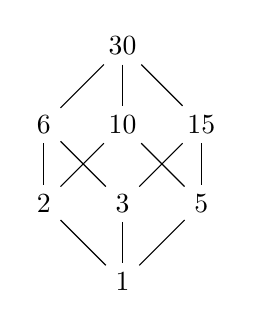
\begin{tikzpicture}[node distance=1cm]
                    \node (1) {30};
                    \node (2) [below of=1] {10};
                    \node (3) [left of=2] {6};
                    \node (4) [right of=2] {15};
                    \node (5) [below of=3] {2};
                    \node (6) [below of=2] {3};
                    \node (7) [below of=4] {5};
                    \node (8) [below of=6] {1};
                    
                    \draw (1) -- (2);
                    \draw (1) -- (3);
                    \draw (1) -- (4);
                    \draw (5) -- (8);
                    \draw (6) -- (8);
                    \draw (7) -- (8);
                    \draw (5) -- (3);
                    \draw (5) -- (2);
                    \draw (6) -- (3);
                    \draw (6) -- (4);
                    \draw (7) -- (2);
                    \draw (7) -- (4);
                \end{tikzpicture}
                \caption{Diagragama de Hasse para $D(30)$.}
            \end{figure}
        \item Para $\cc{B}^3$, el álgebra de Boole con 3 elementos, tenemos:
            \begin{figure}[H]
                \centering
                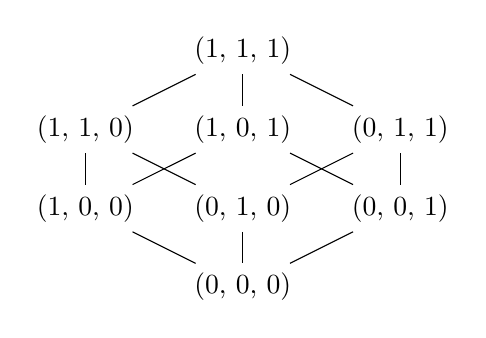
\begin{tikzpicture}[node distance=1cm]
                    \node (1) {(1, 1, 1)};
                    \node (3) [below of=1] {(1, 0, 1)};
                    \node (2) [left of=3, xshift=-1cm] {(1, 1, 0)};
                    \node (4) [right of=3, xshift=1cm] {(0, 1, 1)};
                    \node (5) [below of=2] {(1, 0, 0)};
                    \node (6) [below of=3] {(0, 1, 0)};
                    \node (7) [below of=4] {(0, 0, 1)};
                    \node (8) [below of=6] {(0, 0, 0)};
                    
                    \draw (1) -- (2);
                    \draw (1) -- (3);
                    \draw (1) -- (4);
                    \draw (5) -- (8);
                    \draw (6) -- (8);
                    \draw (7) -- (8);
                    \draw (5) -- (3);
                    \draw (5) -- (2);
                    \draw (6) -- (4);
                    \draw (7) -- (3);
                    \draw (6) -- (2);
                    \draw (7) -- (4);
                \end{tikzpicture}
                \caption{Diagragama de Hasse para $\cc{B}^3$.}
            \end{figure}
    \end{enumerate}
\end{ejemplo}

Centrándonos ya en los retículos que nos interesan, daremos a continuación varios ejemplos de retículos formados por los subgrupos de un grupo dado, que representaremos mediante sus diagramas de Hasse (en estos aparecerán las aristas etiquetadas con números, que por ahora ignoraremos, pero que luego señalaremos lo que significan).

\begin{ejemplo}
    Veamos varios ejemplos con grupos de la forma $\mathbb{Z}_n$:
    \begin{enumerate}
        \item Para calcular el retículo de subgrupos de $\mathbb{Z}_4$, hemos de pensar primero en todos los subgrupos posibles de $\mathbb{Z}_4$. Para ello\footnote{Al final del tema se entenderá por qué es suficiente con esto.}, vemos que:
            \begin{align*}
                \langle {0} \rangle &= \{{0}\} \\
                \langle {1} \rangle &= \mathbb{Z}_4 \\
                \langle {2} \rangle &= \{{0},{2}\} \\
                \langle {3} \rangle &= \mathbb{Z}_4 
            \end{align*}
            Concluimos que $\Lambda_{\mathbb{Z}_4} = \{\{{0}\}, \{{0},{2}\}, \mathbb{Z}_4\}$. Pasamos ahora a ver cómo se relacionan mediante su diagrama de Hasse.
            \begin{figure}[H]
                \centering
                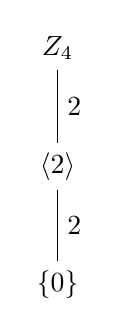
\begin{tikzpicture}[node distance=1.5cm]
                    \node (Z4) {$\bb{Z}_4$};
                    \node (2) [below of=Z4] {$\langle 2 \rangle$};
                    \node (0) [below of=2] {$\{0\}$};

                    \draw (Z4) -- node[right] {$2$} (2);
                    \draw (2) -- node[right] {$2$}(0);
                \end{tikzpicture}
                \caption{Diagrama de Hasse para los subgrupos de $\mathbb{Z}_4$.}
                \label{fig:hasse_z4}
            \end{figure}
        \item En $\mathbb{Z}_6$ tenemos que\footnote{Hemos escrito directamente los subgrupos de $\mathbb{Z}_6$, pero lo que hemos hecho para buscarlos todos es pensar en todos los posibles conjuntos de generadores.}:
            \begin{align*}
                \langle {1} \rangle  = \langle {5} \rangle  &= \mathbb{Z}_6 \\
                \langle {2} \rangle = \langle {4} \rangle  &= \{0, 2, 4\} \\
                \langle {3} \rangle  &= \{0,3\} \\
            \end{align*}
            Y podemos dibujar su diagrama de Hasse:

            \begin{figure}[H]
                \centering
                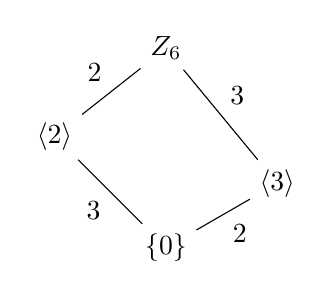
\begin{tikzpicture}[node distance=2cm]
                    \node (Z6) {$\bb{Z}_6$};
                    \node (2) [below left of=Z6, yshift=.3cm] {$\langle 2 \rangle$};
                    \node (3) [below right of=Z6, yshift=-.3cm] {$\langle 3 \rangle$};
                    \node (0) [below right of=2] {$\{0\}$};

                    \draw (Z6) -- node[above left] {$2$} (2);
                    \draw (Z6) -- node[above right] {$3$} (3);
                    \draw (2) -- node[below left] {$3$} (0);
                    \draw (3) -- node[below right] {$2$} (0);
                \end{tikzpicture}
                \caption{Diagrama de Hasse para los subgrupos de $\mathbb{Z}_6$.}
                \label{fig:hasse_z6}
            \end{figure}

        \item En $\mathbb{Z}_8$, tenemos que:
            \begin{align*}
                \langle 1 \rangle  = \langle 3 \rangle  = \langle 5 \rangle  = \langle 7 \rangle  &= \mathbb{Z}_8 \\
                \langle 2 \rangle = \langle 6 \rangle  &= \{0,2,4,6\} \\
                \langle 4 \rangle  &= \{0,4\}
            \end{align*}
            \begin{figure}[H]
                \centering
                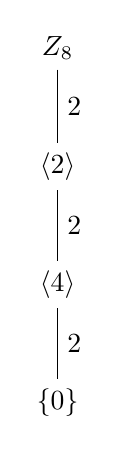
\begin{tikzpicture}[node distance=1.5cm]
                    \node (Z8) {$\bb{Z}_8$};
                    \node (2) [below of=Z8] {$\langle 2 \rangle$};
                    \node (4) [below of=2] {$\langle 4 \rangle$};
                    \node (0) [below of=4] {$\{0\}$};

                    \draw (Z8) -- node[right] {$2$} (2);
                    \draw (2) -- node[right] {$2$}(4);
                    \draw (4) -- node[right] {$2$}(0);
                \end{tikzpicture}
                \caption{Diagrama de Hasse para los subgrupos de $\mathbb{Z}_8$.}
                \label{fig:hasse_z8}
            \end{figure}
        \item En $\mathbb{Z}_{12}$, tenemos:
            \begin{align*}
                \langle 1 \rangle  = \langle 5 \rangle  = \langle 7 \rangle  = \langle 11 \rangle &= \mathbb{Z}_{12}\\
                \langle 2 \rangle   = \langle 10 \rangle &= \{0,2,4,6,8,10\}  \\
                \langle 3 \rangle   = \langle 9 \rangle &= \{0,3,6,9\}  \\
                \langle 4 \rangle  = \langle 8 \rangle&= \{0,4,8\}  \\
                \langle 6 \rangle &= \{0,6\}
            \end{align*}
            \begin{figure}[H]
                \centering
                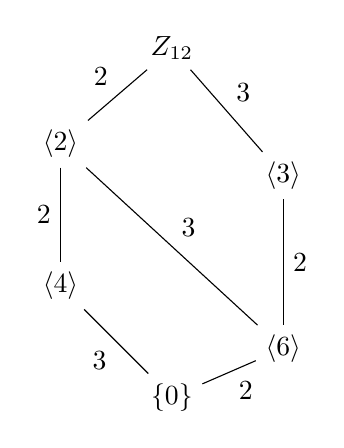
\begin{tikzpicture}[node distance=2cm]
                    \node (Z12) {$\bb{Z}_{12}$};
                    \node (2) [below left of=Z12, yshift=.2cm] {$\langle 2 \rangle$};
                    \node (3) [below right of=Z12, yshift=-.2cm] {$\langle 3 \rangle$};
                    \node (4) [below of=2, yshift=.2cm] {$\langle 4 \rangle$};
                    \node (6) [below of=3, yshift=-.2cm] {$\langle 6 \rangle$};
                    \node (0) [below right of=4] {$\{0\}$};

                    \draw (Z12) -- node[above left] {$2$} (2);
                    \draw (Z12) -- node[above right] {$3$} (3);
                    \draw (2) -- node[left] {$2$} (4);
                    \draw (3) -- node[right] {$2$} (6);
                    \draw (4) -- node[below left] {$3$} (0);
                    \draw (6) -- node[below right] {$2$} (0);
                    \draw (2) -- node[above right] {$3$} (6);
                \end{tikzpicture}
                \caption{Diagrama de Hasse para los subgrupos de $\mathbb{Z}_{12}$.}
                \label{fig:hasse_z12}
            \end{figure}
    \end{enumerate}
\end{ejemplo}

\begin{ejemplo}
    Si trabajamos ahora con otro tipo de grupos:
    \begin{enumerate}
        \item Si consideramos el grupo de Klein:
            \begin{equation*}
                V = \{1, (1\ 2)(3\ 4), (1\ 3)(2\ 4), (1\ 4)(2\ 3)\}
            \end{equation*}
            Todos sus subgrupos posibles son:
            \begin{equation*}
                V, \langle (1\ 2)(3\ 4) \rangle , \langle (1\ 3)(2\ 4) \rangle , \langle (1\ 4)(2\ 3) \rangle , \{1\}
            \end{equation*}

            \begin{figure}[H]
                \centering
                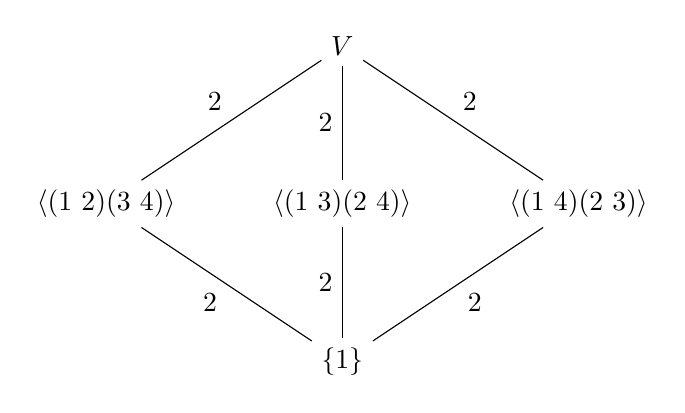
\begin{tikzpicture}[node distance=2cm]
                    \node (V) {$V$};
                    \node (1) [below of=V, xshift=-3cm] {$\left\langle (1\ 2)(3\ 4)\right\rangle$};
                    \node (2) [below of=V] {$\left\langle (1\ 3)(2\ 4)\right\rangle$};
                    \node (3) [below of=V, xshift=3cm] {$\left\langle (1\ 4)(2\ 3)\right\rangle$};
                    \node (4) [below of=2] {$\{1\}$};

                    \draw (V) -- node[above left] {$2$} (1);
                    \draw (V) -- node[left] {$2$} (2);
                    \draw (V) -- node[above right] {$2$} (3);
                    \draw (1) -- node[below left] {$2$} (4);
                    \draw (2) -- node[left] {$2$} (4);
                    \draw (3) -- node[below right] {$2$} (4);
                \end{tikzpicture}    
                \caption{Diagrama de Hasse para los subgrupos del grupo de Klein.}
                \label{fig:hasse_klein}
            \end{figure}

        \item En el grupo de los cuaternios:
            \begin{equation*}
                Q_2 = \{\pm 1,\pm i, \pm j, \pm k\}
            \end{equation*}
            Los subgrupos posibles son:
            \begin{equation*}
                Q_2, \langle i \rangle , \langle j \rangle , \langle k \rangle , \langle -1 \rangle , \{1\}
            \end{equation*}

            \begin{figure}[H]
                \centering
                \begin{tikzpicture}[node distance=2cm]
                    \node (Q2) {$Q_2$};
                    \node (1) [below of=Q2, xshift=-2cm] {$\left\langle i\right\rangle$};
                    \node (2) [below of=Q2] {$\left\langle j\right\rangle$};
                    \node (3) [below of=Q2, xshift=2cm] {$\left\langle k\right\rangle$};
                    \node (4) [below of=2] {$\left\langle -1\right\rangle$};
                    \node (5) [below of=4] {$\{1\}$};

                    \draw (Q2) -- node[above left] {$2$} (1);
                    \draw (Q2) -- node[left] {$2$} (2);
                    \draw (Q2) -- node[above right] {$2$} (3);
                    \draw (1) -- node[below left] {$2$} (4);
                    \draw (2) -- node[left] {$2$} (4);
                    \draw (3) -- node[below right] {$2$} (4);
                    \draw (4) -- node[left] {$2$} (5);
                \end{tikzpicture}
                \caption{Diagrama de Hasse para los subgrupos del grupo de los cuaternios.}
                \label{fig:hasse_cuaternios}
            \end{figure}

        \item En $S_3= \{1, (1\ 2), (1\ 3), (2\ 3), (1\ 2\ 3), (1\ 3\ 2)\}$, los posibles subgrupos son:
            \begin{equation*}
                S_3, \langle (1\ 2\ 3) \rangle , \langle (1\ 2) \rangle , \langle (1\ 3) \rangle , \langle (2\ 3) \rangle , \{1\}
            \end{equation*}

            \begin{figure}[H]
                \centering
                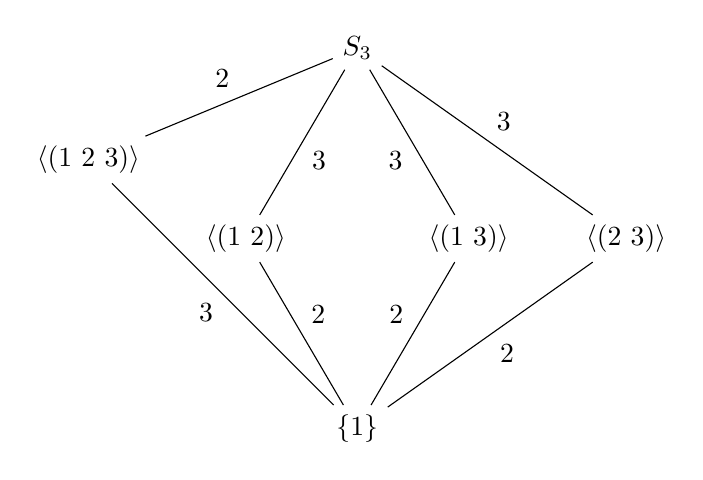
\begin{tikzpicture}[node distance=2cm]
                    \node (S3) {$S_3$};
                    \node (1) [below left of=S3, yshift=-1cm] {$\left\langle (1\ 2)\right\rangle$};
                    \node (2) [below right of=S3, yshift=-1cm] {$\left\langle (1\ 3)\right\rangle$};
                    \node (3) [left of=1, yshift=1cm] {$\left\langle (1\ 2\ 3)\right\rangle$};
                    \node (4) [right of=2] {$\left\langle (2\ 3)\right\rangle$};
                    \node (5) [below right of=1, yshift=-1cm] {$\{1\}$};
                    
                    \draw (S3) -- node[below right] {$3$} (1);
                    \draw (S3) -- node[below left] {$3$} (2);
                    \draw (S3) -- node[above left] {$2$} (3);
                    \draw (S3) -- node[above right] {$3$} (4);
                    \draw (1) -- node[above right] {$2$} (5);
                    \draw (2) -- node[above left] {$2$} (5);
                    \draw (3) -- node[below left] {$3$} (5);
                    \draw (4) -- node[below right] {$2$} (5);
                \end{tikzpicture}
                \caption{Diagrama de Hasse para los subgrupos de $S_3$.}
                \label{fig:hasse_s3}
            \end{figure}

        \item En $D_4= \{1, r, r^2, r^3, s, sr, sr^2, sr^3\}$, los posibles subgrupos son:
            \begin{align*}
                \langle r \rangle  = \langle r^3 \rangle &= \{1, r, r^2, r^3\} \\
                \langle r^2 \rangle  &= \{1, r^2\} \\
                \langle s \rangle  &= \{1, s\} \\
                \langle sr \rangle  &= \{1, sr\} \\
                \langle sr^2 \rangle  &= \{1, sr^2\} \\
                \langle sr^3 \rangle  &= \{1, sr^3\} \\
                \langle r^2, s \rangle  &= \{1, r^2, s, sr^2\} \\
                \langle r^2, sr \rangle  &= \{1, r^2, sr, sr^3\}
            \end{align*}

            \begin{figure}[H]
                \centering
                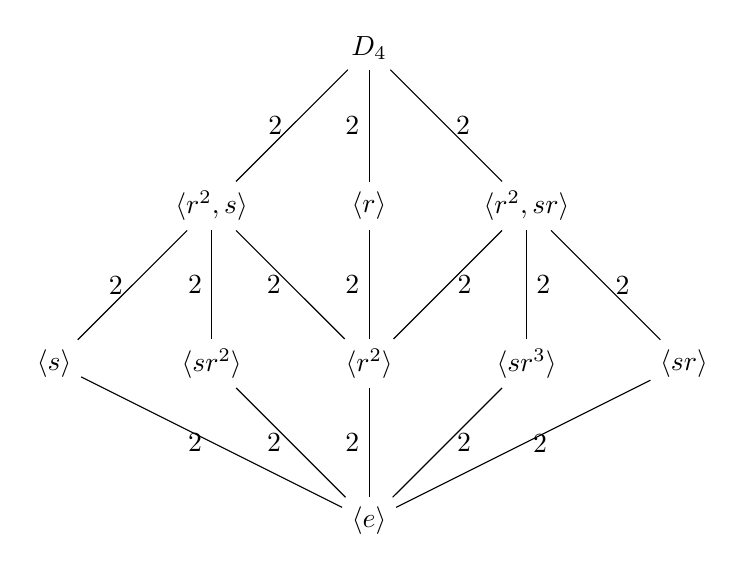
\begin{tikzpicture}[node distance=2cm]
                    \node (D4) {$D_4$};
                    \node[below of=D4] (r) {$\langle r\rangle$};
                    \node[left of=r] (r2s) {$\langle r^2,s\rangle$};
                    \node[right of=r] (r2sr) {$\langle r^2,sr\rangle$};
                    \node[below of=r] (r2) {$\langle r^2\rangle$};
                    \node[left of=r2] (sr2) {$\langle sr^2\rangle$};
                    \node[right of=r2] (sr3) {$\langle sr^3\rangle$};
                    \node[right of=sr3] (sr) {$\langle sr\rangle$};
                    \node[left of=sr2] (s) {$\langle s\rangle$};
                    \node[below of=r2] (1) {$\langle e\rangle$};

                    \draw (D4) --node[left] {$2$} (r);
                    \draw (D4) --node[left] {$2$} (r2s);
                    \draw (D4) --node[right] {$2$} (r2sr);
                    \draw (r) --node[left] {$2$} (r2);
                    \draw (r2s) --node[left] {$2$} (sr2);
                    \draw (r2s) --node[left] {$2$} (s);
                    \draw (r2s) --node[left] {$2$} (r2);
                    \draw (r2sr) --node[right] {$2$} (sr3);
                    \draw (r2sr) --node[right] {$2$} (sr);
                    \draw (r2sr) --node[right] {$2$} (r2);
                    \draw (r2) --node[left] {$2$} (1);
                    \draw (sr2) --node[left] {$2$} (1);
                    \draw (sr3) --node[right] {$2$} (1);
                    \draw (sr) --node[right] {$2$} (1);
                    \draw (s) --node[left] {$2$} (1);
                \end{tikzpicture}
                \caption{Diagrama de Hasse para los subgrupos de $D_4$.}
                \label{fig:hasse_d4}
            \end{figure}
    \end{enumerate}
\end{ejemplo}

\begin{ejemplo}
    Obtenemos un ejemplo interesante al considerar los grupos:
    \begin{align*}
        G &= \langle x,y \mid x^8=y^2=1, xy=yx \rangle \\
        H &= \langle u,v \mid u^2 = v^8 = 1, vu = uv^5 \rangle 
    \end{align*}
    Donde $H$ recibe el nombre de ``grupo modular de orden 16'', notemos que ambos grupos tienen orden 16. En general, si consideramos dos grupos isomorfos, obtendremos dos diagramas de Hasse que serán grafos isomorfos entre sí. Sin embargo, el recíproco no es cierto, si tenemos dos diagramas de Hasse que sean grafos isomorfos, los grupos de los que partían no tienen por qué ser isomorfos. En este ejemplo se pone de manifiesto, ya que $G$ y $H$ no son isomorfos (basta con observar que $G$ es conmutativo y $H$ no), pero veremos que tienen diagramas de Hasse isomorfos. Antes de ello, debemos calcular todos los subgrupos de cada uno, cosa que no vamos a detallar pero sí daremos aquellos subgrupos más grandes:
    \begin{itemize}
        \item $G$ tiene 3 subgrupos de orden 8: $\langle x^2,y \rangle $, $\langle x \rangle $, $\langle xy \rangle $.
        \item $H$ tiene 3 subgrupos de orden 8: $\langle u, v^2 \rangle $, $\langle u \rangle $, $\langle uv \rangle $.
    \end{itemize}

\begin{figure}[H]
    \centering
    \begin{tikzpicture}[node distance=2cm]
        \node (G) {$G$};
        \node (xy) [below of=G] {$\langle xy \rangle$};
        \node (x) [left of=xy] {$\langle x \rangle$};
        \node (x2y) [right of=xy] {$\langle x^2,y \rangle$};
        \node (x2) [below of=xy] {$\langle x^2 \rangle$};
        \node (x2_y) [right of=x2] {$\langle x^2y \rangle$};
        \node (x4y) [right of=x2_y] {$\langle x^4,y \rangle$};
        \node (x4) [below of=x2_y] {$\langle x^4 \rangle$};
        \node (x4_y) [right of=x4] {$\langle x^4y \rangle$};
        \node (y) [right of=x4_y] {$\langle y \rangle$};
        \node (1) [below of=x4_y] {$\{1\}$};

        \draw (G) -- (xy);
        \draw (G) -- (x);
        \draw (G) -- (x2y);
        \draw (x) -- (x2);
        \draw (xy) -- (x2);
        \draw (x2y) -- (x2);
        \draw (x2y) -- (x4y);
        \draw (x2y) -- (x2_y);
        \draw (x2) -- (x4);
        \draw (x2_y) -- (x4);
        \draw (x4y) -- (x4);
        \draw (x4y) -- (x4_y);
        \draw (x4y) -- (y);
        \draw (x4) -- (1);
        \draw (x4_y) -- (1);
        \draw (y) -- (1);
    \end{tikzpicture}
    \caption{Diagrama de Hasse para los subgrupos de $G$.}
\end{figure}

\begin{figure}[H]
    \centering
   \begin{tikzpicture}[node distance=2cm]
        \node (G) {$H$};
        \node (xy) [below of=G] {$\langle uv \rangle$};
        \node (x) [left of=xy] {$\langle v \rangle$};
        \node (x2y) [right of=xy] {$\langle u,v^2 \rangle$};
        \node (x2) [below of=xy] {$\langle v^2 \rangle$};
        \node (x2_y) [right of=x2] {$\langle uv^2 \rangle$};
        \node (x4y) [right of=x2_y] {$\langle u,v^4 \rangle$};
        \node (x4) [below of=x2_y] {$\langle v^4 \rangle$};
        \node (x4_y) [right of=x4] {$\langle uv^4 \rangle$};
        \node (y) [right of=x4_y] {$\langle u \rangle$};
        \node (1) [below of=x4_y] {$\{1\}$};

        \draw (G) -- (xy);
        \draw (G) -- (x);
        \draw (G) -- (x2y);
        \draw (x) -- (x2);
        \draw (xy) -- (x2);
        \draw (x2y) -- (x2);
        \draw (x2y) -- (x4y);
        \draw (x2y) -- (x2_y);
        \draw (x2) -- (x4);
        \draw (x2_y) -- (x4);
        \draw (x4y) -- (x4);
        \draw (x4y) -- (x4_y);
        \draw (x4y) -- (y);
        \draw (x4) -- (1);
        \draw (x4_y) -- (1);
        \draw (y) -- (1);
    \end{tikzpicture} 
    \caption{Diagrama de Hasse para los subgrupos de $H$.}
\end{figure}
\end{ejemplo}

A lo largo de todos estos ejemplos hemos debido darnos cuenta de una particularidad, que se pone de manifiesto especialmente en el ejemplo de los $\mathbb{Z}_n$. Resulta que los órdenes de los subgrupos que hemos ido obteniendo dividían al orden del grupo, resultado que luego demostraremos en general. Sin embargo, estamos ya en condiciones de demostrar que el contrarrecíproco no es cierto en general, es decir, no todos los divisores del orden de un grupo se corresponden con el orden de algún subgrupo suyo.

\begin{prop} 
    El orden del subgrupo divide al orden del grupo, pero no todos los divisores del orden del grupo se corresponden con el orden de algún subgrupo suyo.
\end{prop}
Veremos que el orden de todo subgrupo divide al orden del grupo (en caso de ser el grupo finito) en el Teorema de Lagrange (Teorema~\ref{teo:lagrange}).

\begin{ejemplo}\label{ejemplo:subgrupos_a4}
    Para ver que el recíproco no se cumple, consideramos:
    \begin{multline*}
        A_4 = \{1, (1\ 2)(3\ 4), (1\ 3)(2\ 4), (1\ 4)(2\ 3), (1\ 2\ 3), (1\ 2\ 4), (1\ 3\ 4), (2\ 3\ 4), (1\ 3\ 2),\\ (1\ 4\ 2), (1\ 4\ 3), (2\ 4\ 3)\}
    \end{multline*}
    Que recordamos tiene de orden:
    \begin{equation*}
        |A_4| = \dfrac{4!}{2} = 4\cdot 3 = 12
    \end{equation*}
    Y todos los posibles divisores de $12$ son:
    \begin{equation*}
        D(12) = \{1, 2, 3, 4, 6, 12\}
    \end{equation*}
    Sin embargo, $A_4$ tiene:
    \begin{itemize}
        \item Un subgrupo de orden 1, $\{1\}$.
        \item Cuatro subgrupos de orden 3.
        \item Un subgrupo de orden 4, $V < A_4$.
        \item Tres subgrupos de orden 2.
        \item Un subgrupo de orden 12, $A_4$.
    \end{itemize}
    Más aún, veamos que es imposible que tenga un subgrupo de orden 6.

    \begin{proof}
        Supongamos que existe $H < A_4$ de forma que $|H| = 6$. En dicho caso, viendo todos los elementos de $A_4$, concluimos que $H$ debe contener al menos un $3-$ciclo: 
        \begin{equation*}
            (x_1\ x_2\ x_3) \in  H
        \end{equation*}
        En dicho caso, por ser $H$ un subgrupo de $A_4$, también debe estar su elemento inverso:
        \begin{equation*}
            (x_1\ x_3\ x_2) \in H
        \end{equation*}
        Ahora, distingamos casos:
        \begin{itemize}
            \item Si $H$ no tiene más $3-$ciclos, la única posibilidad (observando nuevamente todos los elementos de $A_4$) es que $H$ sea de la forma:
                \begin{equation*}
                    H = \{1, (1\ 2)(3\ 4), (1\ 3)(2\ 4), (1\ 4)(2\ 3), (x_1\ x_2\ x_3), (x_1\ x_3\ x_2)\}
                \end{equation*}
                En cuyo caso, observemos que $V < H$. Sin embargo, $|V| = 4 \nmid 6 = |H|$, \underline{contradicción}.
            \item Si $H$ tiene otro $3-$ciclo, por ejemplo $(x_1\ x_2\ x_4)$, también ha de contener a su inverso, por lo que:
                \begin{equation*}
                    \{(x_1\ x_2\ x_3), (x_1\ x_3\ x_2), (x_1\ x_2\ x_4), (x_1\ x_4\ x_2)\} \subseteq H
                \end{equation*}
                Sin embargo, como:
                \begin{equation*}
                    (x_1\ x_2\ x_3)(x_1\ x_4\ x_2) = (x_1\ x_4\ x_3)
                \end{equation*}
                Concluimos que también $(x_1\ x_4\ x_3)$ y su inverso: $(x_1\ x_3\ x_4)$ deben estar en $H$, luego $H$ es un subgrupo formado por 6 $3-$ciclos, \underline{contradicción}, ya que $H$ debe también contener al 1.
        \end{itemize}
        Concluimos que no puede existir un subgrupo de $A_4$ con 6 elementos.
    \end{proof}
\end{ejemplo}

\section{Índice y Teorema de Lagrange}
\begin{definicion} % // TODO: Quizás lo muevo antes de comenzar el punto 2.2.
    Sea $G$ un grupo, $H, K < G$, definimos:
    \begin{equation*}
        HK = \{hk \mid h\in H, k \in K\}
    \end{equation*}
\end{definicion}

\begin{prop}\label{prop:hk_kh}
    Sea $G$ un grupo, $H, K < G$, tenemos que $HK$ es un subgrupo de $G$ si y solo si $HK = KH$. En cuyo caso, tendremos que:
    \begin{equation*}
        HK = H\lor K
    \end{equation*}
    \begin{proof}
        Por doble implicación:
        \begin{description}
            \item [$\Longrightarrow)$]   Veamos que $KH = HK$ por doble inclusión:
                \begin{description}
                    \item [$\subseteq)$] Sean $k\in K, h\in H$, tenemos que:
                        \begin{equation*}
                            kh = {(h^{-1}k^{-1})}^{-1} \in HK \Longrightarrow KH \subseteq HK
                        \end{equation*}
                    \item [$\supseteq)$] Observemos que la única hipótesis que tenemos es que $HK$ es un subgrupo de $G$ (nada tenemos sobre $KH$). Sean $h\in H, k\in K$:
                        \begin{equation*}
                            hk = {(k^{-1}h^{-1})}^{-1} \in HK
                        \end{equation*}
                        Por lo que $k^{-1}h^{-1}\in HK$, luego existirán $h_1\in H$, $k_1\in K$ de forma que:
                        \begin{equation*}
                            k^{-1}h^{-1} = h_1k_1
                        \end{equation*}
                        Finalmente:
                        \begin{equation*}
                            hk = {(k^{-1}h^{-1})}^{-1} = {(h_1k_1)}^{-1} = k_1^{-1}h_1^{-1}\in KH
                        \end{equation*}
                \end{description}

            \item [$\Longleftarrow)$] Sean $ hk, h_1k_1 \in HK$, queremos ver qué pasa con $hk{(h_1k_1)}^{-1}$:
                \begin{equation*}
                    hk{(h_1k_1)}^{-1} = h k k_1^{-1} h_1^{-1} \AstIg h k_2 h_2 \stackrel{(\ast\ast)}{=} hh_3k_3 \in HK
                \end{equation*}
                Donde:
                \begin{itemize}
                    \item En $(\ast)$ hemos aplicado que $K$ es un grupo, ya que si $k,k_1\in K$, entonces $kk_1^{-1}\in K$, por lo que existirá $k_2 = kk_1^{-1} \in K$.

                        De forma análoga, como $h_1\in H$, tenemos que $h_1^{-1}\in H$, por lo que existirá $h_2 = h_1^{-1}\in H$.
                    \item En $(\ast\ast)$ hemos aplicado que $k_2h_2 \in KH = HK$, por lo que existirán $h_3 \in H$, $k_3 \in K$ de forma que $k_2h_2 = h_3k_3$.
                \end{itemize}
        \end{description}
        Falta ver que si $HK < G$ con $HK = KH$ (que ya sabemos que son equivalentes), entonces:
        \begin{equation*}
            HK = H\lor K
        \end{equation*}
        \begin{description}
            \item [$\subseteq)$] Sea $x\in HK$, entonces $\exists h\in H, k\in K$ de forma que $x = hk\in \langle H\cup K \rangle = H\lor K$. 
            \item [$\supseteq)$] Sea $x\in H\lor K$, entonces sabemos que existen $\alpha_1,\ldots,\alpha_n \in H\cup K$ y $\gamma_1,\ldots,\gamma_n\in \mathbb{Z}$ de forma que:
                \begin{equation*}
                    x = \alpha_1^{\gamma_1}\ldots\alpha_n^{\gamma_n}
                \end{equation*}
                Como $HK = KH$, tras varias conmutaciones de términos, existirán ${h_1,\ldots,h_p \in H}$, $k_{p+1},\ldots,k_n\in K$ y $\delta_1,\ldots,\delta_n\in \mathbb{Z}$ de forma que:
                \begin{equation*}
                    x = h_1^{\delta_1}\ldots h_p^{\delta_p}k_{p+1}^{\delta_{p+1}}\ldots k_n^{\delta_n}
                \end{equation*}
                Y por ser $H$ y $K$ grupos, tendremos que:
                \begin{align*}
                    h &= h_1^{\delta_1}\ldots h_p^{\delta_p} \in H \\
                    k &= k_{p+1}^{\delta_{p+1}}\ldots k_n^{\delta_n} \in K
                \end{align*}
                Por lo que $x=hk \in HK$. \qedhere
        \end{description}
    \end{proof}
\end{prop}

\begin{definicion}
    Sea $G$ un grupo y $H < G$, definimos dos relaciones binarias en $G$:
    \begin{itemize}
        \item La relación $\prescript{}{H}{\sim}$ definida por:
            \begin{equation*}
                y \prescript{}{H}{\sim\ } x \Longleftrightarrow x^{-1}y\in H
            \end{equation*}
        \item La relación $\sim_H$ definida por:
            \begin{equation*}
                y\sim_H x \Longleftrightarrow yx^{-1} \in  H
            \end{equation*}
    \end{itemize}
\end{definicion}

\begin{prop}
    Sea $G$ un grupo y $H < G$, se verifica que $\prescript{}{H}{\sim}$ y $\sim_H$ son relaciones de equivalencia en $G$. Además, dado $x\in G$, se tiene que sus clases de equivalencia\footnote{Que denotaremos por $\prescript{}{H}{[x]}$ y por $[x]_H$ respectivamente.} son de la forma:
    \begin{align*}
        \prescript{}{H}{[x]} &= \{xh \mid h\in H\} \\
        [x]_H &= \{hx \mid h\in H\}
    \end{align*}
    \begin{proof}
        Comprobemos primero que $\prescript{}{H}{\sim}$ y $\sim_H$ son relaciones de equivalencia:
        \begin{itemize}
            \item \underline{Propiedad reflexiva.} Como $H$ es un grupo, $1\in H$, por lo que dado $x\in G$:
                \begin{equation*}
                    xx^{-1} = x^{-1}x = 1 \in H
                \end{equation*}
                De donde deducimos que $x\sim_H x$ y $x\prescript{}{H}{\sim\ }x$, de forma respectiva.
            \item \underline{Propiedad simétrica.} Sean $x,y\in G$:
                \begin{itemize}
                    \item Si $x\prescript{}{H}{\sim\ } y$, entonces $y^{-1}x \in H$, pero por ser $H$ un grupo, también tendremos:
                        \begin{equation*}
                            {(y^{-1}x)}^{-1} = x^{-1}y \in H
                        \end{equation*}
                        De donde deducimos que $y\prescript{}{H}{\sim\ } x$.
                    \item Si $x\sim_H y$, entonces $xy^{-1}\in H$, y por ser $H$ un grupo:
                        \begin{equation*}
                            {(xy^{-1})}^{-1} = yx^{-1}\in H
                        \end{equation*}
                        De donde deducimos que $y\sim_H x$.
                \end{itemize}
            \item \underline{Propiedad transitiva.} Sean $x,y,z\in G$:
                \begin{itemize}
                    \item Si $x\prescript{}{H}{\sim\ } y$ y $y\prescript{}{H}{\sim\ } z$, entonces: $y^{-1}x, z^{-1}y \in H$ y por ser $H$ un grupo, deducimos que:
                        \begin{equation*}
                            (z^{-1}y)(y^{-1}x) = z^{-1}x \in H
                        \end{equation*}
                        De donde $x\prescript{}{H}{\sim\ } z$.
                    \item Si $x\sim_H y$ y $y\sim_H z$, entonces $xy^{-1},yz^{-1}\in H$ y por ser $H$ un grupo:
                        \begin{equation*}
                            (xy^{-1})(yz^{-1}) = xz^{-1} \in H
                        \end{equation*}
                        De donde $x\sim_H z$.
                \end{itemize}
        \end{itemize}
        Concluimos que $\prescript{}{H}{\sim\ }$ y $\sim_H$ son relaciones de equivalencia en $G$. Falta comprobar las igualdades:
    \begin{align*}
        \prescript{}{H}{[x]} &\stackrel{(1)}{=} \{xh \mid h\in H\} \\
        [x]_H &\stackrel{(2)}{=} \{hx \mid h\in H\}
    \end{align*}
    \begin{enumerate}
        \item Sean $x,y\in G$, tenemos que:
            \begin{align*}
                x\prescript{}{H}{\sim\ } y &\Longleftrightarrow y^{-1}x \in H \Longleftrightarrow \exists h\in H \text{\ con\ } y^{-1}x = h \Longleftrightarrow \exists h\in H \text{\ con\ } y^{-1} = hx^{-1} \\
                                           &\Longleftrightarrow \exists h\in H \text{\ con\ } y=xh^{-1} \Longleftrightarrow \exists h'\in H\text{\ con\ } y = xh'
            \end{align*}
            Concluimos que se cumple $(1)$.
        \item Sean $x,y\in G$:
            \begin{align*}
                x\sim_H y &\Longleftrightarrow xy^{-1}\in  H \Longleftrightarrow \exists h\in H \text{\ con\ } xy^{-1} = h \Longleftrightarrow \exists h\in H \text{\ con\ } y = h^{-1}x \\
                          &\Longleftrightarrow \exists h'\in H \text{\ con\ } y=hx
            \end{align*}
            Concluimos que también se cumple $(2)$.
    \end{enumerate}
    \end{proof}
\end{prop}

\begin{definicion}
    Sea $G$ un grupo y $H < G$:
    \begin{itemize}
        \item Si consideramos la relación $\prescript{}{H}{\sim}$, dado $x\in G$, definimos la clase lateral por la izquierda de $G$ en $H$ definida por $x$ a la clase de equivalencia de $x$ por la relación de equivalencia $\prescript{}{H}{\sim}$, que denotamos por:
            \begin{equation*}
                xH = \{xh\mid h \in H\}
            \end{equation*}
            De esta forma, tendremos que el conjunto cociente dado por la relación es de la forma:
            \begin{equation*}
                G/\prescript{}{H}{\sim\ } = \{xH \mid x\in G\}
            \end{equation*}
        \item Si consideramos ahora la relación $\sim_H$, dado $x\in G$, definimos la clase lateral por la derecha de $G$ en $H$ definida por $x$ a la clase de equivalencia de $x$ por la relación de equivalencia $\sim_H$, denotada por:
            \begin{equation*}
                Hx = \{hx\mid h\in H\}
            \end{equation*}
            Y consideraremos el conjunto cociente:
            \begin{equation*}
                G/\sim_H = \{Hx \mid x \in G\}
            \end{equation*}
    \end{itemize}
\end{definicion}

\begin{ejemplo}
    En $S_3 = \{1, (1\ 2), (1\ 3), (2\ 3), (1\ 2\ 3), (1\ 3\ 2)\}$, si consideramos como $H$:
    \begin{equation*}
        H = \langle (1\ 2) \rangle  = \{1, (1\ 2)\}
    \end{equation*}
    Podemos calcular todas las clases laterales por la izquierda de $G$ en $H$ si consideramos la relación $\prescript{}{H}{\sim}$:
    \begin{align*}
        1H &= \{1\cdot 1, 1(1\ 2)\} = \{1, (1\ 2)\} = H \\
        (1\ 2)H &= \{(1\ 2)1, (1\ 2)(1\ 2)\} = \{(1\ 2), 1\} = H \\
        (1\ 3)H &= \{(1\ 3)1, (1\ 3)(1\ 2)\} = \{(1\ 3), (1\ 2\ 3)\} \\
        (2\ 3)H &= \{(2\ 3)1, (2\ 3)(1\ 2)\} = \{(2\ 3), (1\ 3\ 2)\} \\
        (1\ 2\ 3)H &= \{(1\ 2\ 3)1, (1\ 2\ 3)(1\ 2)\} = \{(1\ 2\ 3), (1\ 3)\} = (1\ 3)H \\
        (1\ 3\ 2)H &= \{(1\ 3\ 2)1, (1\ 3\ 2)(1\ 2)\} = \{(1\ 3\ 2), (2\ 3)\} = (2\ 3)H
    \end{align*} 
    Por lo que el conjunto cociente $G/\prescript{}{H}{\sim}$ vendrá dado por:
    \begin{equation*}
        G/\prescript{}{H}{\sim} = \{H, (1\ 3)H, (2\ 3)H\}
    \end{equation*}
    Si ahora calculamos todas las clases laterales por la derecha de $G$ en $H$, considerando la relación $\sim_H$, entonces:
    \begin{align*}
        H1 &= \{1\cdot 1, (1\ 2)1\} = \{1, (1\ 2)\} = H \\
        H(1\ 2) &= \{1(1\ 2), (1\ 2)(1\ 2)\} = \{(1\ 2), 1\} = H \\
        H(1\ 3) &= \{1(1\ 3), (1\ 2)(1\ 3)\} = \{(1\ 3), (1\ 3\ 2)\} \\
        H(2\ 3) &= \{1(2\ 3), (1\ 2)(2\ 3)\} = \{(2\ 3), (1\ 2\ 3)\} \\
        H(1\ 2\ 3) &= \{1(1\ 2\ 3), (1\ 2)(1\ 2\ 3)\} = \{(1\ 2\ 3), (2\ 3)\} = H(2\ 3) \\
        H(1\ 3\ 2) &= \{1(1\ 3\ 2), (1\ 2)(1\ 3\ 2)\} = \{(1\ 3\ 2), (1\ 3)\} = H(1\ 3)
    \end{align*}
    Por lo que el conjunto cociente $G/\sim_H$ vendrá dado por:
    \begin{equation*}
        G/\sim_H = \{H, H(1\ 3), H(2\ 3)\}
    \end{equation*}
\end{ejemplo}

\begin{prop}\label{prop:biyecciones_conj_cocientes}
    Sea $G$ un grupo, $H < G$ y $x\in G$, entonces:
    \begin{enumerate}
        \item[$i)$] $x\in xH$ y $x\in Hx$.
        \item[$ii)$] Los conjuntos $H$, $xH$ y $Hx$ son biyectivos.
        \item[$iii)$] Los conjuntos cocientes $G/\prescript{}{H}{\sim}$ y $G/\sim_H$ son biyectivos.
    \end{enumerate}
    \begin{proof} Veamos cada una de ellas:
        \begin{enumerate}
            \item[$i)$] Como $H$ es un grupo, tendremos que $1\in H$, por lo que:
                \begin{equation*}
                    x = x\cdot 1 \in xH \qquad x = 1\cdot x \in Hx
                \end{equation*}
            \item[$ii)$] Sean $f:xH\longrightarrow H$, $g:H\longrightarrow Hx$ dadas por:
                \begin{align*}
                    f(xh) &= h \qquad \forall xh\in xH \\
                    g(h) &= hx \qquad \forall h\in H
                \end{align*}
                Es fácil comprobar que $f$ y $g$ son biyectivas, por lo que $xH$ es biyectivo con $H$ y $H$ es biyectivo con $Hx$. Basta considerar $g\circ f$ para obtener una biyección de $xH$ con $Hx$.
            \item[$iii)$] Sea $f:G/\prescript{}{H}{\sim}\longrightarrow G/\sim_H$ dada por:
                \begin{equation*}
                    f(xH) = Hx^{-1} \qquad \forall xH \in G/\prescript{}{H}{\sim}
                \end{equation*}
                En primer lugar, hemos de ver que $f$ está bien definida. Para ello, sean $x,y\in G$ de forma que $xH = yH$, entonces $x\prescript{}{H}{\sim\ } y$, luego $y^{-1}x\in H$, pero por ser $H$ un grupo:
                \begin{equation*}
                    {(y^{-1}x)}^{-1} = x^{-1}y \in H \Longrightarrow x^{-1}\sim_H y^{-1}
                \end{equation*}
                Por lo que $Hx^{-1} = Hy^{-1}$, luego $f$ está bien definida. Finalmente, es fácil ver que $f$ es biyectiva. \qedhere
        \end{enumerate}
    \end{proof}
\end{prop}

\begin{definicion}[Índice de un grupo en un subgrupo]
    Sea $G$ un grupo y $H<G$, en la Proposición~\ref{prop:biyecciones_conj_cocientes}, vimos que:
    \begin{equation*}
        |G/\prescript{}{H}{\sim}| = |G/\sim_H|
    \end{equation*}
    Los cardinales de estos conjuntos recibirán el nombre de \underline{índice de $G$ en $H$}, y los denotaremos por $[G:H]$.
\end{definicion}

\begin{ejemplo}
    En los diagramas de Hasse de las Figuras~\ref{fig:hasse_z4},~\ref{fig:hasse_z6},~\ref{fig:hasse_z8},~\ref{fig:hasse_z12},~\ref{fig:hasse_klein},~\ref{fig:hasse_cuaternios},~\ref{fig:hasse_s3} y~\ref{fig:hasse_d4}, los números que dibujábamos en las aristas de los diagramas de Hasse eran los índices de los grupos en los respectivos subgrupos marcados por la arista. Por ejemplo, en la Figura~\ref{fig:hasse_s3}, observamos que $[S_3:\langle (1\ 2) \rangle ] = 3$, algo que comprobamos en el último ejemplo, donde tomábamos:
    \begin{equation*}
        H = \langle (1\ 2) \rangle  = \{1, (1\ 2)\}
    \end{equation*}
    En esta situación, teníamos que $[S_3:H] = |G/\sim_H| = |G/\prescript{}{H}{\sim}| = 3$.
\end{ejemplo}

\begin{teo}[de Lagrange]\label{teo:lagrange} % // TODO: Candidato a caer en examenes
    Sea $G$ un grupo finito y $H < G$, entonces:
    \begin{equation*}
        |G| = [G:H]|H|
    \end{equation*}
    Observemos que a partir de esta igualdad deducimos que $|H|$ divide a $|G|$.
    \begin{proof}
        Como $\prescript{}{H}{\sim}$ es una relación de equivalencia, tenemos una partición de $G$ a partir de las clases de equivalencia dadas por esta relación:
        \begin{equation*}
            G = \bigcup_{x\in G} xH
        \end{equation*}
        Como $G$ es finito, habrá un número finito de clases de equivalencia. Si elegimos un elemento en cada una de estas, tendremos un conjunto con cada uno de los representantes de las clases $\{x_1, x_2, \ldots, x_n\}$, con lo que:
        \begin{equation*}
            |G| = |x_1H| + |x_2H| + \ldots + |x_nH| \AstIg n|H|
        \end{equation*}
        Donde en $(\ast)$ hemos usado la Proposición~\ref{prop:biyecciones_conj_cocientes}, ya que como $xH$ es biyectivo con $H$ para cualquier $x\in G$, concluimos que $|x_iH| = |x_1H|$ para todo $i \in \{1,\ldots,n\}$. Sin embargo, $n$ es el número de clases de equivalencia distintas del conjunto cociente, es decir, $n=[G:H]$, con lo que:
        \begin{equation*}
            |G| = [G:H]|H|
        \end{equation*}
    \end{proof}
\end{teo}

\begin{observacion}
    Notemos que a partir del Teorema de Lagrange podemos deducir resultados ya vistos y demostrados, como por ejemplo, la Proposición~\ref{prop:orden_sl}, donde deducíamos el orden de los grupos $|\SL_n(\bb{F})|$, pero resulta que $[\GL_n(\bb{F}):\SL_n(\bb{F})] = q-1$ si $|\bb{F}| = q$, por lo que:
    \begin{equation*}
        |\GL_n(\bb{F})| = (q-1)|\SL_n(\bb{F})|
    \end{equation*}
\end{observacion}

\begin{coro}
    Sea $G$ un grupo finito, el orden de cualquier elemento de $G$ divide a $|G|$.
    \begin{proof}
        Sea $x\in G$, basta ver que $O(x) = |\langle x \rangle |$. Sin embargo, por la Proposición~\ref{prop:orden_grupo}, ya vimos que por ser $G$ un grupo finito, entonces $\exists n\in \mathbb{N}\setminus\{0\}$ de forma que $O(x) = n$. En esta misma Proposición vimos que entonces $x$ tenía $n$ potencias distintas, por lo que:
        \begin{equation*}
            \langle x \rangle  = \{1,x,x^2,\ldots,x^{n-1}\} \Longrightarrow |\langle x \rangle | = n
        \end{equation*}
        Basta aplicar el Teorema de Lagrange, puesto que $\langle x \rangle < G$.
    \end{proof}
\end{coro}

\begin{coro}
    Sea $G$ un grupo finito y $K < H < G$, entonces:
    \begin{equation*}
        [G:K] = [G:H][H:K]
    \end{equation*}
    \begin{proof}
        Por el Teorema de Lagrange, sabemos que:
        \begin{equation*}
            \left.\begin{array}{r}
                    |G| = [G:K]|K| \\
                    |G| = [G:H]|H| = [G:H][H:K]|K|
            \end{array}\right\} \Longrightarrow [G:K] = [G:H][H:K]
        \end{equation*}
    \end{proof}
\end{coro}

\section{Propiedades de grupos cíclicos}
Terminaremos este capítulo repasando varias propiedades de los grupos cíclicos que debemos conocer, no sin antes recordar la definición de un grupo cíclico. Decimos que un grupo $G$ es cíclico si $\exists a\in G$ de forma que $G = \langle a \rangle $. En cuyo caso, todos los elementos de $G$ serán potencias de $a$: si $x\in G$, existirá $n\in \mathbb{Z}$ de forma que $x=a^n$.\\

Antes de continuar, recordamos una propiedad de los grupos cíclicos: sea $G = \langle a \rangle $ un grupo cíclico, entonces:
\begin{equation*}
    |G| = O(a)
\end{equation*}

\begin{prop}\label{prop:grupo_primo}
    Si $G$ es un grupo con $|G|=p$ primo, entonces $G$ es cíclico.
    \begin{proof}
        Sea $a\in G$, $a\neq 1$ (como $p$ es primo, $p\geq 2$), observamos que:
        \begin{equation*}
            \{1\} \neq \langle a \rangle < G
        \end{equation*}
        Por el Teorema de Lagrange, $1\neq |\langle a \rangle | $ divide a $|G|$, pero $p$ es primo, por lo que $|\langle a \rangle | = p$ y ha de ser $\langle a \rangle = G$.
    \end{proof}
\end{prop}

\begin{lema}
    Sea $G$ un grupo, $a\in G$, existe un homomorfismo de grupos 
    \begin{equation*}
        \varphi_a:\mathbb{Z}\to G
    \end{equation*}
    De forma que $\varphi_a(1) = a$ y $Im(\varphi_a) = \{a^n \mid n \in \mathbb{Z}\} = \langle a \rangle$.
    \begin{proof}
        Definimos $\varphi_a$ como la aplicación:
        \begin{equation*}
            \varphi_a(n) = a^n \qquad \forall n\in \mathbb{Z}
        \end{equation*}
        Es claro que $\varphi_a(1)=a$ y que $Im(\varphi_a) = \{a^n \mid n\in \mathbb{Z}\} = \langle a \rangle $. Falta ver que $\varphi_a$ es un homomorfismo. Para ello:
        \begin{equation*}
            \varphi_a(n+m) = a^{n+m} = a^n a^m = \varphi_a(n)\varphi_a(m) \qquad \forall n,m\in \mathbb{Z}
        \end{equation*}
    \end{proof}
\end{lema}

\begin{teo}\label{teo:grupos_ciclicos}
    Sea $G$ un grupo cíclico, entonces:
    \begin{itemize}
        \item Si $G$ es infinito, $G\cong \mathbb{Z}$.
        \item Si $|G| = n$, $G\cong \mathbb{Z}_n$.
    \end{itemize}
    \begin{proof}
        Como $G$ es cíclico, existirá $a\in G$ de forma que $\langle a \rangle = G$. El Lema anterior nos da una aplicación $\varphi_a:\mathbb{Z}\to G$ sobreyectiva, veamos cómo conseguir la inyectividad:
        \begin{itemize}
            \item \underline{Si $G$ es infinito}, entonces ha de ser $O(a)=+\infty$, por lo que $\nexists n\in \mathbb{N}\setminus\{0\}$ de forma que $\varphi_a(n) = a^n = 1$, por lo que:
                \begin{equation*}
                    \ker(\varphi_a) = \{0\} \Longrightarrow \varphi_a \text{\ inyectiva}
                \end{equation*}
                Concluimos que $G\cong \mathbb{Z}$.
            \item \underline{Si $G$ es finito} y tiene cardinal $n\in \mathbb{N}\setminus\{0\}$, entonces tendremos que $O(a) = n$, por lo que $\varphi_a(n) = a^n = 1$ y $\varphi_a$ no será inyectiva por ser $\{0,n\}\subseteq \ker(\varphi_a)$. Sin embargo, podemos definir la aplicación $\psi_a:\mathbb{Z}_n\to G$ dada por $\psi_a(\overline{r}) = a^r$ para todo $\overline{r}\in \mathbb{Z}_n$:
                \begin{itemize}
                    \item $\psi_a$ está bien definida, ya que si $\overline{r},\overline{s}\in \mathbb{Z}_n$ de forma que $\overline{r}=\overline{s}$, entonces:
                        \begin{equation*}
                            r-s\in n\mathbb{Z} \Longrightarrow \exists t\in \mathbb{Z} \text{\ con\ }  a^{r-s} = a^{nt} = {(a^n)}^{t} = 1 \Longrightarrow a^r = a^s
                        \end{equation*}
                    \item $\psi_a$ es un homomorfismo:
                        \begin{equation*}
                            \psi_a(\overline{r}+\overline{s}) = a^{r+s} = a^r a^s = \psi_a(\overline{r})\psi_a(\overline{s}) \qquad \forall \overline{r},\overline{s}\in \mathbb{Z}_n
                        \end{equation*}
                    \item $\psi_a$ es inyectiva, ya que si $\overline{r}\in \mathbb{Z}_n$ con $\psi_a(\overline{r}) = a^r = 1$, entonces $n\mid r$, luego $\overline{r} = \overline{0}$ y se tiene que:
                        \begin{equation*}
                            \ker(\psi_a) = \{\overline{0}\}
                        \end{equation*}
                    \item Como $\langle a \rangle =G$ y $|G| = n = O(a)$, está claro que $\psi_a$ es sobreyectiva.
                \end{itemize}
                Por todo esto, concluimos que $\psi_a$ es un isomorfismo, luego $G\cong \mathbb{Z}_n$.
        \end{itemize}
    \end{proof}
\end{teo}

% // TODO: Clase

\begin{prop}
    Sea $G=\langle a \rangle $ un grupo cíclico con $O(a) = n$, entonces para cada divisor $m$ de $n$, existe un único subgrupo de $G$ de orden $m$, el subgrupo cíclico $\left\langle a^{\frac{n}{m}} \right\rangle$.
    Además, estos son los únicos subgrupos de $G$. % EJemplo: Z4
    \begin{proof}
        Sea $m$ un divisor de $n$, veamos que $\left\langle a^{\frac{n}{m}} \right\rangle $ es un grupo cíclico de orden $m$. Para ello, veamos que $O\left(a^{\frac{n}{m}}\right) = m$:
        \begin{itemize}
            \item En primer lugar, tenemos que:
                \begin{equation*}
                    {(a^{\frac{n}{m}})}^{m} = a^n = 1
                \end{equation*}
            \item Sea $t\in \mathbb{N}\setminus\{0\}$ de forma que:
                \begin{equation*}
                    {(a^{\frac{n}{m}})}^{t} = 1 \Longrightarrow n \mid \dfrac{nt}{m}
                \end{equation*}
                En cuyo caso, existe $r\in \mathbb{N}$ de forma que:
                \begin{equation*}
                    \dfrac{nt}{m} = rn \Longrightarrow t = rm \Longrightarrow m \mid t
                \end{equation*}
        \end{itemize}
        Concluimos que $O(a^{\frac{n}{m}}) = m$. Ahora, si $H<G$, nos gustaría probar que si $|H| = m$, entonces:
        \begin{equation*}
            m\in Div(n) \quad \text{y} \quad H = \left\langle a^{\frac{n}{m}} \right\rangle 
        \end{equation*}
        En primer lugar, observemos que si $H<G$, por el Teorema de Lagrange tenemos que $m\mid n$. Para ver la igualdad, sea:
        \begin{equation*}
            k = \min\{t\in \mathbb{N}\setminus\{0\}\mid a^t \in H\}
        \end{equation*}
        Veamos que $H = \langle a^k \rangle $:
        \begin{description}
            \item [$\supseteq)$] Se tiene por la definición de $k$.
            \item [$\subseteq)$] Sea $b\in H < G = \langle a \rangle $, entonces $\exists s\in \mathbb{N}$ de forma que $b = a^s$. Si dividimos $s$ entre $k$, tenemos que $\exists q,r\in \mathbb{N}$ de forma que:
                \begin{equation*}
                    s = kq + r \qquad 0\leq r < k
                \end{equation*}
                Y por ser $a^s, a^k\in H$, vemos que:
                \begin{equation*}
                    a^r = a^s a^{-kq} \in H
                \end{equation*}
                Por esto, concluimos que $r=0$, ya que $k$ era el menor natural no nulo que cumplía esta propiedad (y $r<k$), por lo que $s = kq$ y:
                \begin{equation*}
                    b = {(a^k)}^{q} \in \langle a^k \rangle 
                \end{equation*}
        \end{description}
        Falta finalmente ver que $k = \nicefrac{n}{m}$. Para ello, como $a^n = 1 \in H$ por ser $H$ un grupo, tenemos que $k\leq n$ y si dividimos $n$ entre $k$, $\exists q,r \in \mathbb{N}$ de forma que:
        \begin{equation*}
            n = qk + r \qquad 0\leq r < k
        \end{equation*}
        De donde: $1 = a^n = a^{qk}a^r$, pero por ser $1\in H$ y $a^{qk}\in H$, deducimos que $a^r \in H$ con $r<k$, luego ha de ser $r=0$ (ya que si no entraría en contradicción con la definición de $k$), por lo que $k\mid n$. De aquí deducimos que:
        \begin{equation*}
             m = |H| = O(a^k)\AstIg \dfrac{n}{k} \Longrightarrow k = \dfrac{n}{m}
        \end{equation*}
        Donde en $(\ast)$ hemos usado que $O(a^k) = \dfrac{n}{k}$, ya que:
        \begin{itemize}
            \item En primer lugar:
                \begin{equation*}
                    {(a^k)}^{\frac{n}{k}} = a^n = 1
                \end{equation*}
            \item Si $t\in \mathbb{N}$ de forma que:
                \begin{equation*}
                    {(a^k)}^{t} = 1 = a^n
                \end{equation*}
                Como $O(a)=n$, por la Proposición~\ref{prop:divide_orden}, tenemos que $n\mid kt$, luego existe $s$ de forma que:
                \begin{equation*}
                    ns = kt \Longrightarrow \dfrac{n}{k}s = t
                \end{equation*}
                Por lo que $\frac{n}{k}\mid t$.
        \end{itemize}
        Lo que nos dice que $O(a^k) = \dfrac{n}{k}$.
    \end{proof}
\end{prop}

\begin{observacion}
    De la Proposición anterior, deducimos que dado $G$ un grupo cíclico con $|G| = n$, entonces la aplicación $\phi:Div(n)\to \Lambda_G$ con:
    \begin{equation*}
        \Lambda_G = \{H \subseteq G \mid H < G\}
    \end{equation*}
    dada por:
    \begin{equation*}
        \phi(m) = \left\langle a^{\frac{n}{m}} \right\rangle \qquad \forall m\in Div(n)
    \end{equation*}
    Es una biyección.
\end{observacion}

\begin{ejemplo}
    A partir de esta última observación, es muy fácil calcular todos los subgrupos de cualquier grupo cíclico, ya que el problema se reduce a estudiar todos los divisores del orden del grupo. Ilustramos el procedimiento con el grupo cíclico de orden $12$:
    \begin{equation*}
        C_{12} = \langle x\mid x^{12} = 1 \rangle 
    \end{equation*}
    Tenemos que:
    \begin{equation*}
        Div(12) = \{1, 2, 3, 4, 6, 12\}
    \end{equation*}
    Y usando nuestra aplicación $\phi$, podemos listar todos los subgrupos de $C_{12}$:
    \begin{align*}
        1 &\stackrel{\phi}{\longmapsto} \left\langle x^{\frac{12}{1}} \right\rangle = \left\langle x^{12} \right\rangle  = \langle 1 \rangle  = \{1\} \\
        2 &\longmapsto \left\langle x^{\frac{12}{2}} \right\rangle = \langle x^{6} \rangle  = \{1, x^6\} \\
        3 &\longmapsto \left\langle x^{\frac{12}{3}} \right\rangle = \langle x^4 \rangle = \{1, x^4, x^8\} \\
        4 &\longmapsto \left\langle x^{\frac{12}{4}} \right\rangle  = \langle x^3 \rangle = \{1, x^3, x^6, x^9\} \\
        6 &\longmapsto \left\langle x^{\frac{12}{6}} \right\rangle = \langle x^2 \rangle = \{1, x^2, x^4, x^6, x^8, x^{10}\} \\
        12 &\longmapsto \left\langle x^{\frac{12}{12}} \right\rangle = \langle x \rangle  = C_{12}
    \end{align*}
    Por lo que su diagrama de Hasse será de la forma: 
    \begin{figure}[H]
        \centering
        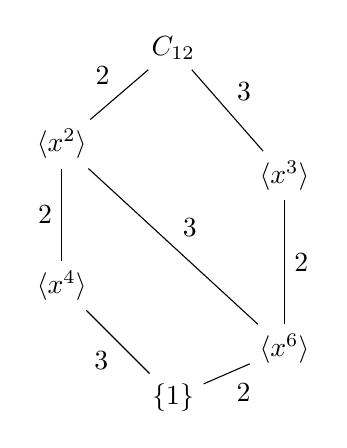
\begin{tikzpicture}[node distance=2cm]
            \node (Z12) {$C_{12}$};
            \node (2) [below left of=Z12, yshift=.2cm] {$\langle x^2 \rangle$};
            \node (3) [below right of=Z12, yshift=-.2cm] {$\langle x^3 \rangle$};
            \node (4) [below of=2, yshift=.2cm] {$\langle x^4 \rangle$};
            \node (6) [below of=3, yshift=-.2cm] {$\langle x^6 \rangle$};
            \node (0) [below right of=4] {$\{1\}$};

            \draw (Z12) -- node[above left] {$2$} (2);
            \draw (Z12) -- node[above right] {$3$} (3);
            \draw (2) -- node[left] {$2$} (4);
            \draw (3) -- node[right] {$2$} (6);
            \draw (4) -- node[below left] {$3$} (0);
            \draw (6) -- node[below right] {$2$} (0);
            \draw (2) -- node[above right] {$3$} (6);
        \end{tikzpicture}
        \caption{Diagrama de Hasse para los subgrupos de ${C}_{12}$.}
        \label{fig:hasse_c12}
    \end{figure}
\end{ejemplo}

\begin{coro}
    Si tenemos un grupo cíclico de orden $p^n$ con $p$ primo, entonces todos sus subgrupos serán cíclicos y de orden $p^r$, con $0\leq r\leq n$.
\end{coro}

\begin{prop}\label{prop:orden_zn}
    Sea $G$ un grupo, $a\in G$ con $O(a) = n$ y $k\in \mathbb{N}\setminus\{0\}$, entonces:
    \begin{equation*}
        \langle a^k \rangle  = \langle a^d \rangle \qquad \text{\ siendo\ } d = \mcd(n,k)
    \end{equation*}
    En cuyo caso, $O(a^k) = \dfrac{n}{d}$.
    \begin{proof}
        Por doble inclusión:
        \begin{description}
            \item [$\subseteq)$] Como $d\mid k$, tenemos que $k = dt$ para cierto $t$, luego $a^k = a^{dt}\in \langle a^d \rangle $.
            \item [$\supseteq)$] Como $d = \mcd(n,k)$, entonces la ecuación:
                \begin{equation*}
                    nX + kY = d
                \end{equation*}
                tiene solución\footnote{Se vió en Álgebra I, se trata de la Identidad de Bezout.}, por lo que existen $u,v\in \mathbb{N}$ de forma que $nu + kv = d$, luego:
                \begin{equation*}
                    a^d = a^{nu}a^{kv} = \cancelto{1}{{(a^n)}^{u}} {(a^{k})}^{v} \in \langle a^k \rangle 
                \end{equation*}
        \end{description}
        Para ver que $O(a^k) = \nicefrac{n}{d}$, como $\left\langle a^k \right\rangle = \left\langle a^d \right\rangle  $, tenemos que $O(a^k) = O(a^d)$ y como:
        \begin{itemize}
            \item Tenemos que:
                \begin{equation*}
                    {(a^d)}^{\frac{n}{d}} = a^n = 1
                \end{equation*}
            \item Si $t\in \mathbb{N}$ de forma que:
                \begin{equation*}
                    {(a^d)}^{t} = 1 \Longrightarrow n \mid dt \Longrightarrow \dfrac{n}{d}\mid t
                \end{equation*}
        \end{itemize}
        Concluimos que $O(a^k) = O(a^d)  = \nicefrac{n}{d} $.
    \end{proof}
\end{prop}

\begin{ejemplo}
    Por ejemplo, ¿por qué en $\mathbb{Z}_{12}$ el subgrupo generado por el 8 coincide con el generado por el 4? Porque $4 = \mcd(8,12)$.
\end{ejemplo}

\begin{coro}
    Sea $G$ un grupo y $a\in G$ con $O(a) = n$, entonces:
    \begin{equation*}
        \langle a^p \rangle  = \langle a^q \rangle  \Longleftrightarrow \mcd(n,p) = \mcd(n,q)
    \end{equation*}
    \begin{proof}
        Veamos la doble implicación:
        \begin{description}
            \item [$\Longleftarrow)$] Si $\mcd(n,p) = d = \mcd(n,q)$, entonces (por la Proposición anterior):
                \begin{equation*}
                    \langle a^p \rangle  = \langle a^d \rangle  = \langle a^q \rangle 
                \end{equation*}
            \item [$\Longrightarrow)$] Si $\langle a^p \rangle = \langle a^q \rangle $, entonces (por la Proposición anterior):
                \begin{equation*}
                    \dfrac{n}{\mcd(n,p)} = O(a^p) = O(a^q) = \dfrac{n}{\mcd(n,q)} \Longrightarrow \mcd(n,p) = \mcd(n,q)
                \end{equation*}
        \end{description}
    \end{proof}
\end{coro}

\begin{coro}
    Sea $G = \langle a \rangle $ un grupo cíclico con $O(a) = n$, entonces:
    \begin{equation*}
        G = \langle a^k \rangle  \Longleftrightarrow \mcd(k,n) = 1
    \end{equation*}
    Es decir, el número de generadores de $G$ es $\varphi(n)$, siendo $\varphi$ la función de Euler:
    \begin{equation*}
        \varphi(n) = |\{m\in \mathbb{N} \mid 1\leq m\leq n \land \mcd(n,m)=1\}|
    \end{equation*}
    \begin{proof}
        Basta usar el Corolario anterior:
        \begin{equation*}
            G = \langle a \rangle = \langle a^k \rangle \Longleftrightarrow 1 = \mcd(n,1) = \mcd(n,k) 
        \end{equation*}
    \end{proof}
\end{coro}

\begin{ejemplo}
    En $\mathbb{Z}_{12}$:
    \begin{equation*}
        \mathbb{Z}_{12} = \langle \overline{1} \rangle  = \langle \overline{5} \rangle  = \langle \overline{7} \rangle  = \langle \overline{11} \rangle 
    \end{equation*}
\end{ejemplo}
